\documentclass[11pt,a4paper]{article}

% ── Packages ──────────────────────────────────────────────
\usepackage[utf8]{inputenc}
\usepackage[T1]{fontenc}
\usepackage{amsmath,amssymb}
\usepackage{graphicx}
\usepackage[margin=2.5cm]{geometry}
\usepackage{booktabs}
\usepackage{caption}
\usepackage{subcaption}
\usepackage{hyperref}
\usepackage{float}

% ── Title ─────────────────────────────────────────────────
\title{Assignment 2: ARMA Processes and Seasonal Processes\\[4pt]
       \large 02417 Time Series Analysis --- DTU}
\author{Student numbers: [INSERT HERE]}
\date{\today}

\begin{document}
\maketitle

%===================================================================
\section{Stability}\label{sec:stability}
%===================================================================

Let the process $\{X_t\}$ be an AR(2) given by
\[
  X_t + \phi_1 X_{t-1} + \phi_2 X_{t-2} = \varepsilon_t,
\]
where $\{\varepsilon_t\}$ is white noise with $\sigma_\varepsilon = 1$,
and $\phi_1 = -0.7$, $\phi_2 = -0.2$.

%-------------------------------------------------------------------
\subsection{Stationarity (1.1)}\label{sec:stationarity}

The characteristic polynomial of the AR(2) process is
\[
  \phi(z) = 1 + \phi_1 z + \phi_2 z^2 = 1 - 0.7z - 0.2z^2.
\]
The process is stationary if and only if all roots of $\phi(z) = 0$ lie
\emph{outside} the unit circle, i.e.\ $|z_i| > 1$ for all roots $z_i$.

Setting $\phi(z) = 0$:
\[
  -0.2z^2 - 0.7z + 1 = 0 \quad\Longleftrightarrow\quad 0.2z^2 + 0.7z - 1 = 0.
\]
Using the quadratic formula:
\[
  z = \frac{-0.7 \pm \sqrt{0.49 + 0.8}}{0.4}
    = \frac{-0.7 \pm \sqrt{1.29}}{0.4}
    = \frac{-0.7 \pm 1.1358}{0.4}.
\]
This gives two real roots:
\[
  z_1 = \frac{-0.7 + 1.1358}{0.4} \approx 1.089, \qquad
  z_2 = \frac{-0.7 - 1.1358}{0.4} \approx -4.589.
\]
Since $|z_1| \approx 1.089 > 1$ and $|z_2| \approx 4.589 > 1$, both roots lie
outside the unit circle, and the process is \textbf{stationary}.

%-------------------------------------------------------------------
\subsection{Invertibility (1.2)}\label{sec:invertibility}

Invertibility requires that all roots of the MA polynomial $\theta(z) = 0$
lie outside the unit circle. For this AR(2) process the MA polynomial is
simply $\theta(z) = 1$ (no MA component), which has no roots. Therefore,
the process is \textbf{trivially invertible}.

More generally, a pure AR process is always invertible because the
$\varepsilon_t$ can already be expressed as a finite linear combination of
present and past $X_t$ values.

%-------------------------------------------------------------------
\subsection{Autocorrelation function (1.3)}\label{sec:acf-formula}

Multiplying the AR equation by $X_{t-k}$ and taking expectations yields the
Yule--Walker equations. For $k \geq 1$:
\[
  \gamma(k) + \phi_1 \gamma(k-1) + \phi_2 \gamma(k-2) = 0,
\]
so, dividing by $\gamma(0)$:
\[
  \rho(k) = -\phi_1\,\rho(k-1) - \phi_2\,\rho(k-2), \qquad k \geq 2.
\]
The initial conditions are $\rho(0) = 1$ and, from the $k=1$ equation:
\[
  \rho(1) + \phi_1 + \phi_2\,\rho(1) = 0
  \quad\Longrightarrow\quad
  \rho(1) = \frac{-\phi_1}{1 + \phi_2}.
\]
Substituting $\phi_1 = -0.7$ and $\phi_2 = -0.2$:
\[
  \rho(1) = \frac{0.7}{0.8} = 0.875.
\]
Subsequent values follow the recursion:
\begin{align*}
  \rho(2) &= -\phi_1\,\rho(1) - \phi_2\,\rho(0)
           = 0.7 \times 0.875 + 0.2 \times 1 = 0.8125, \\
  \rho(3) &= 0.7 \times 0.8125 + 0.2 \times 0.875 = 0.7438, \\
  &\;\vdots
\end{align*}
The ACF decays towards zero without oscillation, consistent with two positive
real reciprocal roots.

%-------------------------------------------------------------------
\subsection{ACF plot (1.4)}\label{sec:acf-plot}

\begin{figure}[H]
  \centering
  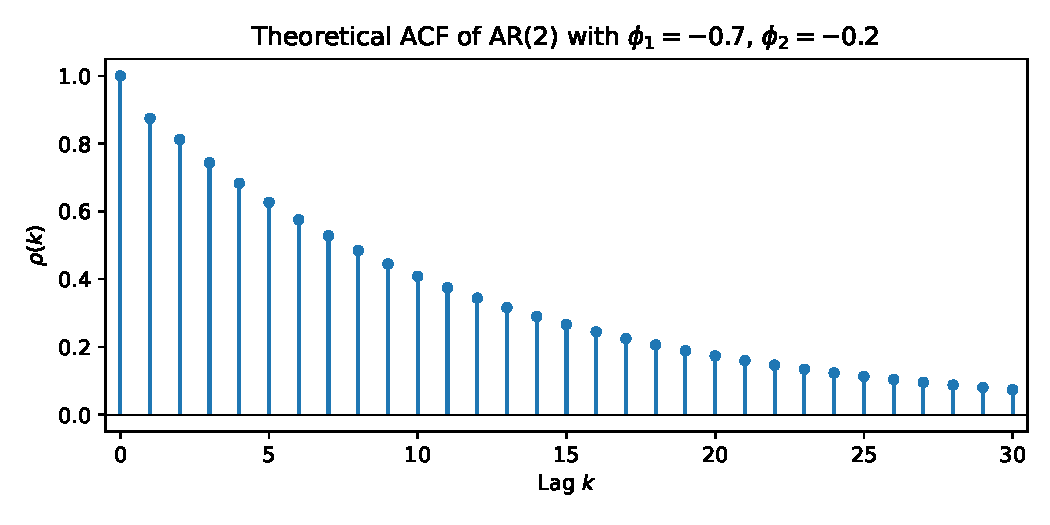
\includegraphics[width=0.85\textwidth]{../plots/sec1_acf.pdf}
  \caption{Theoretical ACF $\rho(k)$ of the AR(2) process for $k = 0,\dots,30$.}
  \label{fig:sec1-acf}
\end{figure}

The ACF decays smoothly towards zero, reflecting the two real roots
$z_1 \approx 1.09$ and $z_2 \approx -4.59$. Because both roots are positive
in reciprocal form (the dominant root $1/z_1 \approx 0.92$ is close to 1),
the decay is slow and essentially monotone.


%===================================================================
\section{Simulating seasonal processes}\label{sec:seasonal}
%===================================================================

A multiplicative $(p,d,q) \times (P,D,Q)_s$ seasonal model is defined by
\[
  \phi(B)\,\Phi(B^s)\,\nabla^d \nabla_s^D\, Y_t
  = \theta(B)\,\Theta(B^s)\,\varepsilon_t,
\]
where $\phi(B)$ and $\theta(B)$ are non-seasonal polynomials of orders $p$ and $q$,
and $\Phi(B^s)$ and $\Theta(B^s)$ are seasonal polynomials in $B^s$.
All models below have $d = D = 0$ and $s = 12$.

For each model we simulate $N = 300$ observations (with a burn-in of 500) and
display the time series, sample ACF, and sample PACF.

%-------------------------------------------------------------------
\subsection{Model 2.1: $(1,0,0)\times(0,0,0)_{12}$, $\phi_1 = 0.6$}

The combined model is simply $\phi(B) Y_t = \varepsilon_t$ with
$\phi(B) = 1 + 0.6\,B$, i.e.\ a non-seasonal AR(1):
\[
  Y_t + 0.6\,Y_{t-1} = \varepsilon_t
  \quad\Longleftrightarrow\quad
  Y_t = -0.6\,Y_{t-1} + \varepsilon_t.
\]

\begin{figure}[H]
  \centering
  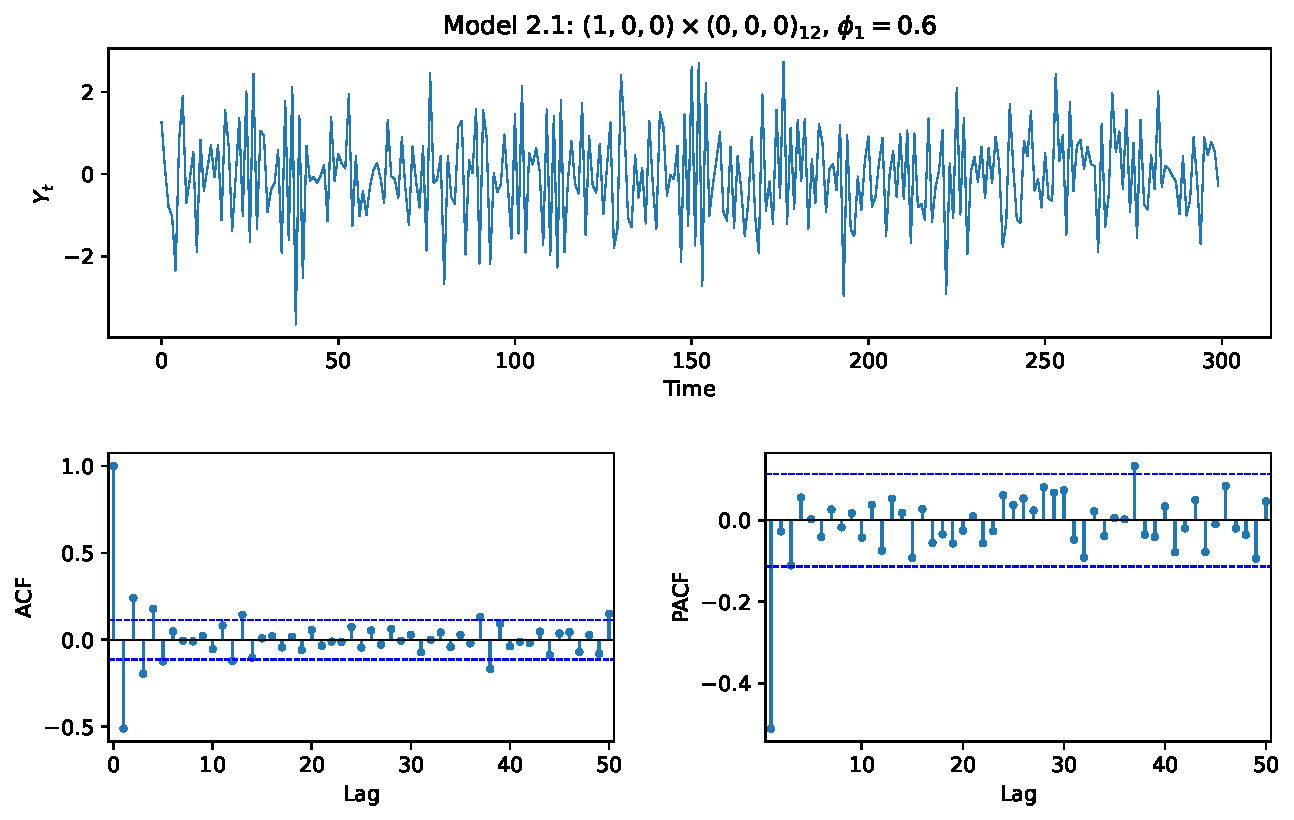
\includegraphics[width=\textwidth]{../plots/sec2_model_2_1.pdf}
  \caption{Model 2.1: AR(1) with $\phi_1 = 0.6$.}
  \label{fig:model21}
\end{figure}

The ACF decays geometrically with alternating sign ($\rho(k) \approx (-0.6)^k$),
which is the hallmark of an AR(1) process with a positive $\phi_1$ in our
convention (corresponding to a negative ``standard'' AR coefficient).
The PACF shows a single significant spike at lag~1 and is zero thereafter,
confirming the AR(1) structure.

%-------------------------------------------------------------------
\subsection{Model 2.2: $(0,0,0)\times(1,0,0)_{12}$, $\Phi_1 = -0.9$}

The model is $\Phi(B^{12}) Y_t = \varepsilon_t$ with
$\Phi(B^{12}) = 1 - 0.9\,B^{12}$:
\[
  Y_t - 0.9\,Y_{t-12} = \varepsilon_t.
\]

\begin{figure}[H]
  \centering
  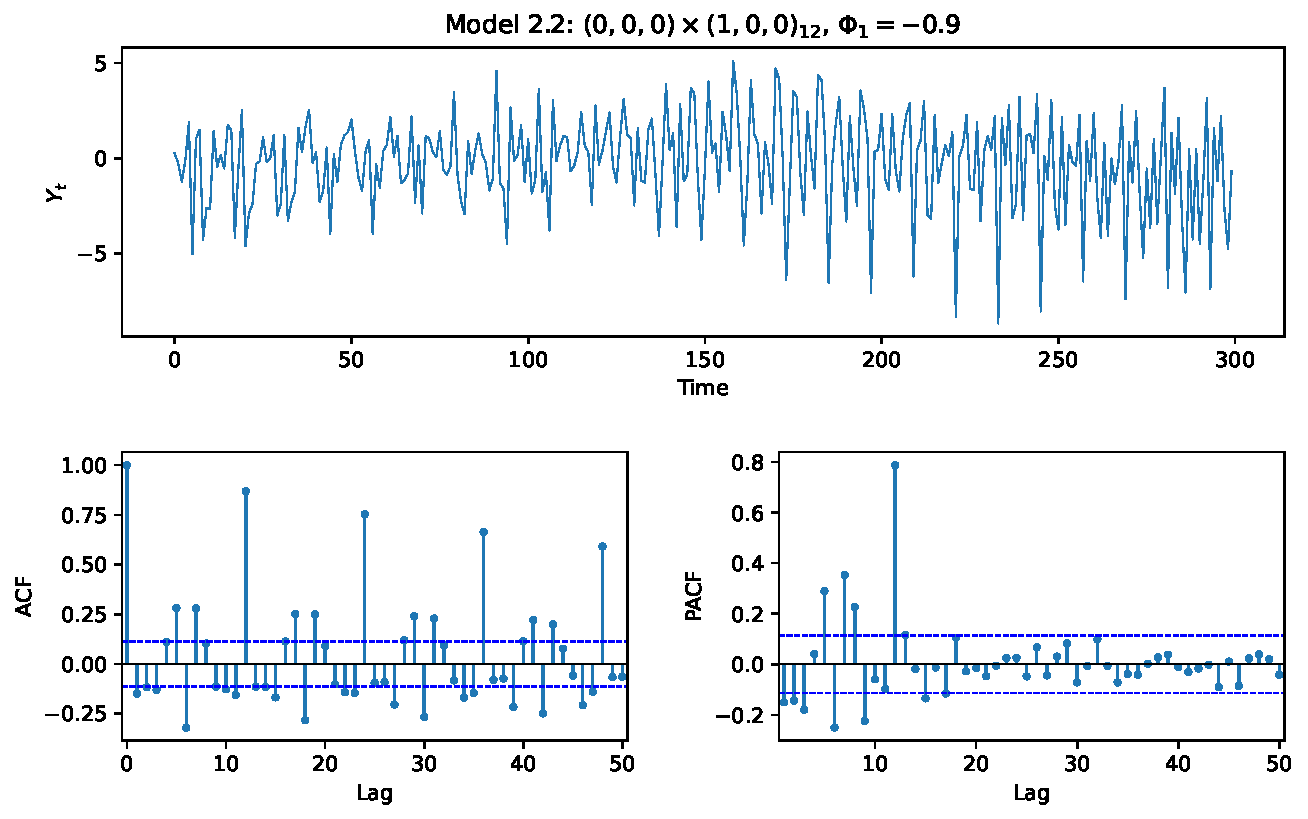
\includegraphics[width=\textwidth]{../plots/sec2_model_2_2.pdf}
  \caption{Model 2.2: Seasonal AR(1)$_{12}$ with $\Phi_1 = -0.9$.}
  \label{fig:model22}
\end{figure}

The time series shows a clear seasonal pattern with period 12.
The ACF displays large spikes at multiples of 12 (lags 12, 24, 36, \ldots)
that decay slowly, reflecting the near-unit-root seasonal AR component
($\Phi_1 = -0.9$).
The PACF has a single significant spike at lag~12 and is essentially zero at
non-seasonal lags, consistent with a purely seasonal AR(1)$_{12}$.

%-------------------------------------------------------------------
\subsection{Model 2.3: $(1,0,0)\times(0,0,1)_{12}$, $\phi_1 = 0.9$, $\Theta_1 = -0.7$}

The combined model is:
\[
  (1 + 0.9\,B)\,Y_t = (1 - 0.7\,B^{12})\,\varepsilon_t.
\]

\begin{figure}[H]
  \centering
  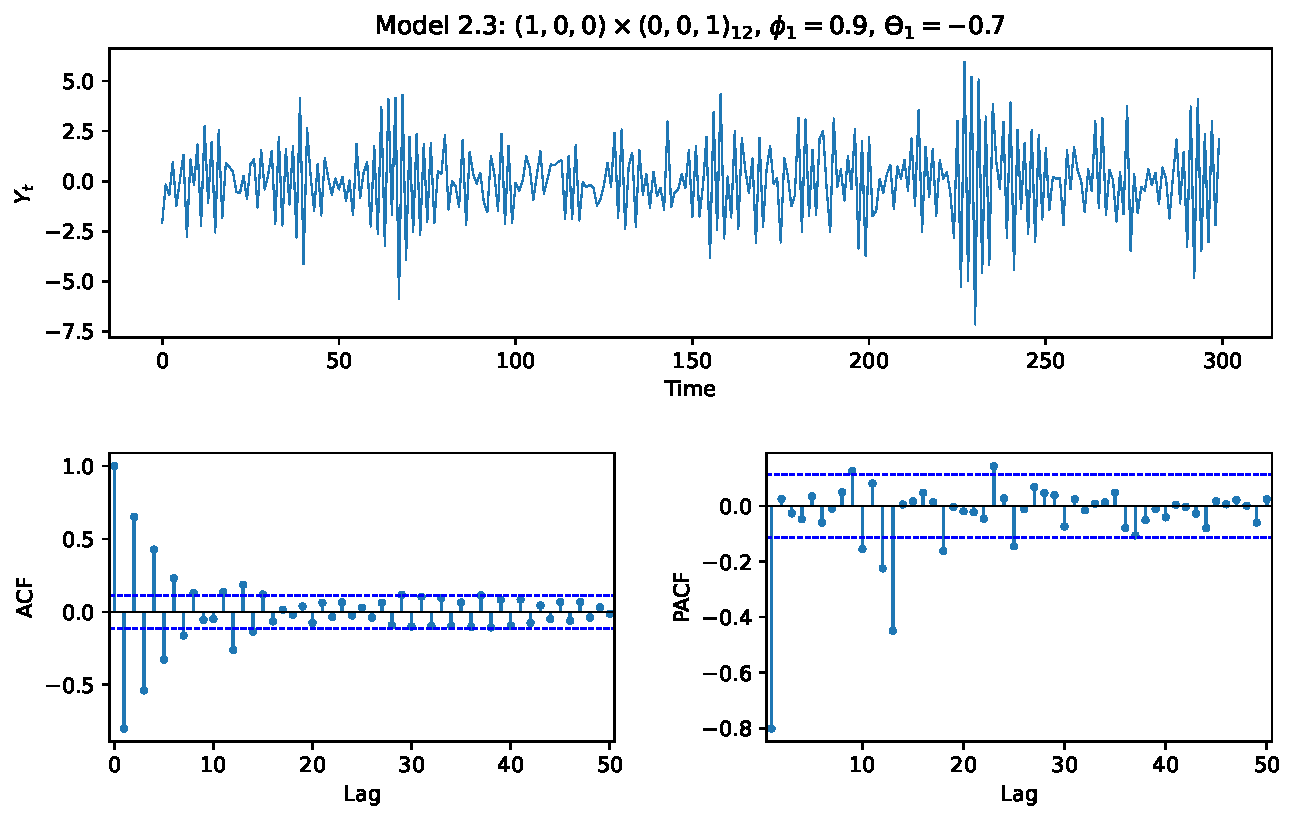
\includegraphics[width=\textwidth]{../plots/sec2_model_2_3.pdf}
  \caption{Model 2.3: AR(1) $\times$ SMA(1)$_{12}$ with $\phi_1 = 0.9$,
           $\Theta_1 = -0.7$.}
  \label{fig:model23}
\end{figure}

The non-seasonal AR(1) component with $\phi_1 = 0.9$ produces alternating-sign
decay in the ACF at short lags. The seasonal MA(1) with $\Theta_1 = -0.7$
introduces a cutoff in the seasonal structure: the ACF shows significant spikes
at lag~12 but not at lag~24. The PACF shows spikes at lag~1 (from the AR part)
and near lag~12 (from the seasonal MA part), with an interaction visible at
lags 11 and 13.

%-------------------------------------------------------------------
\subsection{Model 2.4: $(1,0,0)\times(1,0,0)_{12}$, $\phi_1 = -0.6$, $\Phi_1 = -0.8$}

The combined AR polynomial is:
\[
  (1 - 0.6\,B)(1 - 0.8\,B^{12})
  = 1 - 0.6\,B - 0.8\,B^{12} + 0.48\,B^{13}.
\]

\begin{figure}[H]
  \centering
  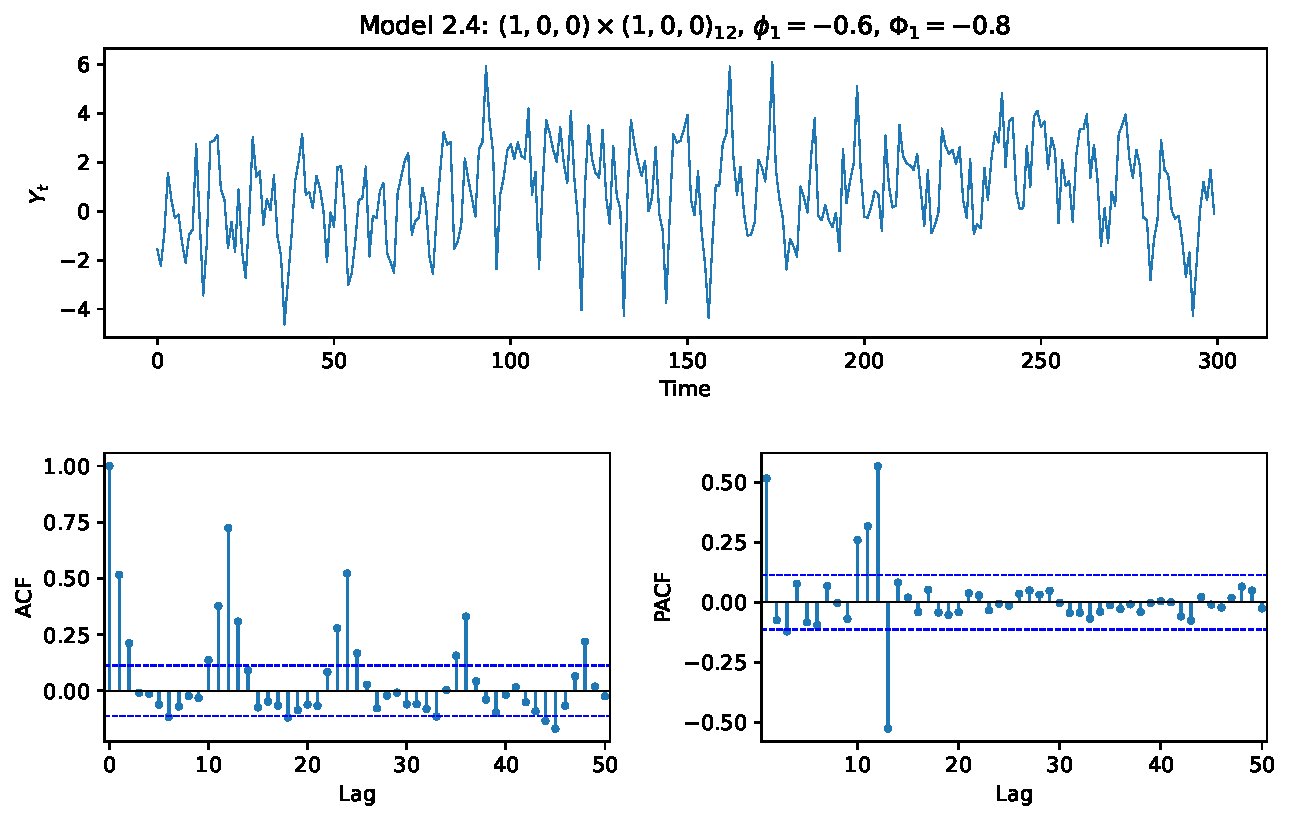
\includegraphics[width=\textwidth]{../plots/sec2_model_2_4.pdf}
  \caption{Model 2.4: AR(1) $\times$ SAR(1)$_{12}$ with $\phi_1 = -0.6$,
           $\Phi_1 = -0.8$.}
  \label{fig:model24}
\end{figure}

The ACF shows slow decay at both short (non-seasonal) lags and at seasonal
lags (12, 24, \ldots). The non-seasonal decay is positive (reflecting
$\phi_1 = -0.6$ in our convention), and the seasonal peaks at lags 12, 24, 36
decay slowly due to the near-unit-root $\Phi_1 = -0.8$.
The PACF exhibits significant spikes at lag~1 (non-seasonal AR) and lag~12
(seasonal AR), with the multiplicative interaction creating additional
structure near lags~11 and~13.

%-------------------------------------------------------------------
\subsection{Model 2.5: $(0,0,1)\times(0,0,1)_{12}$, $\theta_1 = 0.4$, $\Theta_1 = -0.8$}

The combined MA polynomial is:
\[
  (1 + 0.4\,B)(1 - 0.8\,B^{12})
  = 1 + 0.4\,B - 0.8\,B^{12} - 0.32\,B^{13}.
\]

\begin{figure}[H]
  \centering
  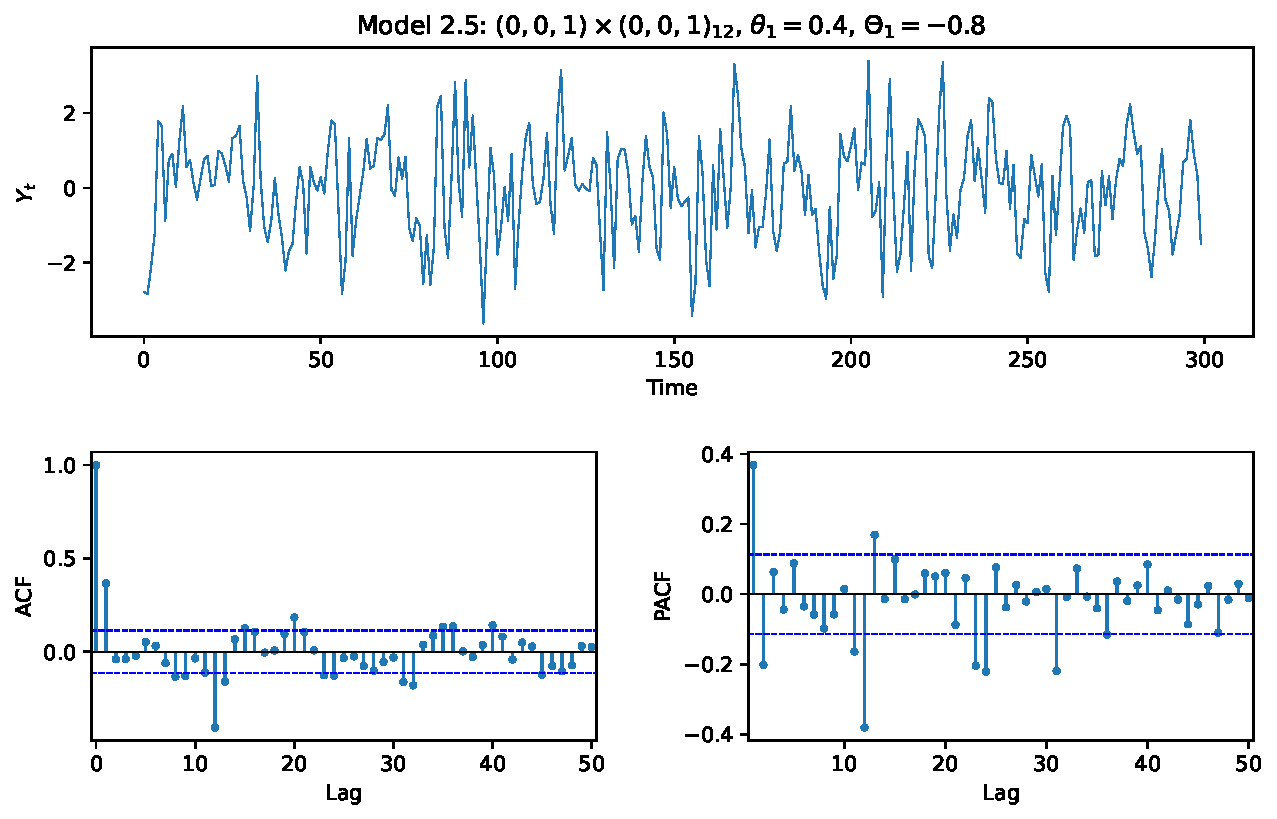
\includegraphics[width=\textwidth]{../plots/sec2_model_2_5.pdf}
  \caption{Model 2.5: MA(1) $\times$ SMA(1)$_{12}$ with $\theta_1 = 0.4$,
           $\Theta_1 = -0.8$.}
  \label{fig:model25}
\end{figure}

This is a purely MA process. The ACF has the characteristic multiplicative MA
fingerprint: significant values only at lags 1, 11, 12, and 13, with all other
lags near zero. Lag~1 reflects the non-seasonal MA, lags~12 reflects the
seasonal MA, and lags~11 and~13 arise from the cross-product
$\theta_1 \cdot \Theta_1$. The PACF shows a more complex decaying pattern,
consistent with a pure MA process (PACF tails off while ACF cuts off).

%-------------------------------------------------------------------
\subsection{Model 2.6: $(0,0,1)\times(1,0,0)_{12}$, $\theta_1 = -0.4$, $\Phi_1 = 0.7$}

The combined model is:
\[
  (1 + 0.7\,B^{12})\,Y_t = (1 - 0.4\,B)\,\varepsilon_t.
\]

\begin{figure}[H]
  \centering
  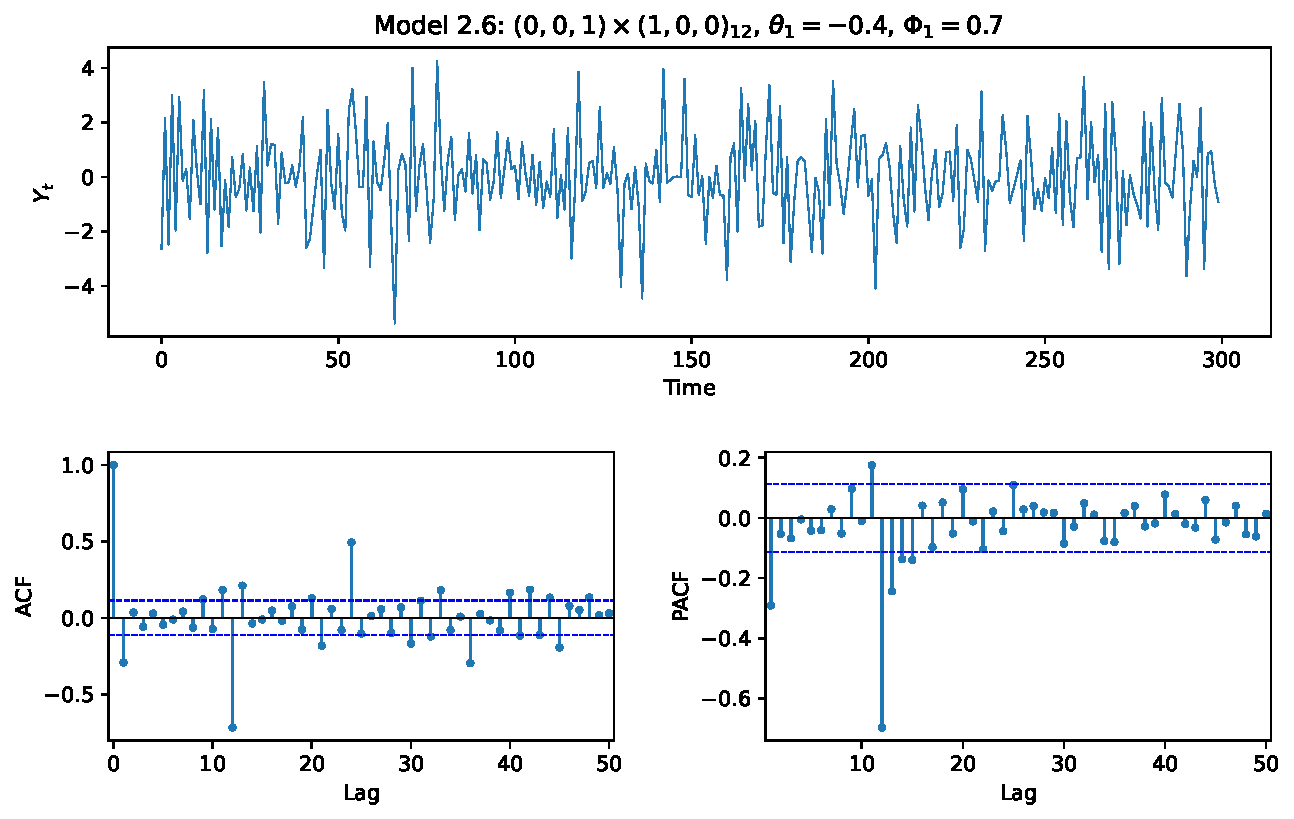
\includegraphics[width=\textwidth]{../plots/sec2_model_2_6.pdf}
  \caption{Model 2.6: MA(1) $\times$ SAR(1)$_{12}$ with $\theta_1 = -0.4$,
           $\Phi_1 = 0.7$.}
  \label{fig:model26}
\end{figure}

The non-seasonal MA(1) produces a sharp cutoff in the ACF after lag~1 at
short lags, while the seasonal AR(1) creates slowly decaying spikes at
seasonal lags (12, 24, 36, \ldots). The PACF shows the combined effect:
a significant spike at lag~1 from the MA interaction, and a pattern of
decaying spikes at multiples of 12 from the seasonal AR component.

%-------------------------------------------------------------------
\subsection{Summary of observations (2.7)}\label{sec:summary}

From the six simulations, we draw the following general conclusions about
the ACF and PACF of seasonal ARMA processes:

\begin{enumerate}
  \item \textbf{Seasonal AR components} ($\Phi$) produce slowly decaying ACF
        values at seasonal lags ($s, 2s, 3s, \ldots$) and a sharp cutoff in
        the PACF at the seasonal lag, mirroring the behaviour of non-seasonal
        AR components at unit lags.

  \item \textbf{Seasonal MA components} ($\Theta$) produce a sharp cutoff in
        the ACF at the seasonal lag (nonzero at lag $s$, zero at $2s, 3s, \ldots$)
        and a decaying pattern in the PACF at seasonal lags.

  \item \textbf{Multiplicative structure} creates interaction between seasonal
        and non-seasonal components. For a multiplicative MA model like
        $(0,0,1)\times(0,0,1)_s$, the ACF is nonzero only at lags $1$,
        $s-1$, $s$, and $s+1$ --- the fingerprint of multiplicative MA.

  \item The seasonal and non-seasonal components act \emph{independently} at
        their respective lag domains: non-seasonal behaviour dominates at
        short lags (1, 2, \ldots), seasonal behaviour dominates at multiples
        of $s$, and interaction effects appear at lags near $s$ (specifically
        $s \pm 1$, $s \pm 2$, etc.).

  \item The identification rules (ACF cutoff $\Rightarrow$ MA; PACF cutoff
        $\Rightarrow$ AR) apply separately at both the non-seasonal and
        seasonal levels, making it possible to identify the orders
        $(p,q)$ and $(P,Q)$ by examining different lag regions.
\end{enumerate}


%===================================================================
\section{Identifying ARMA models}\label{sec:identification}
%===================================================================

%-------------------------------------------------------------------
\subsection{Process 1 (3.1)}

\textbf{Identified model: MA(1).}

The ACF shows a single significant spike at lag~1 ($\approx 0.8$) and then
drops sharply to values within the confidence bands for all subsequent lags.
This cutoff after lag~1 is the defining characteristic of an MA(1) process.
The PACF exhibits a gradual (exponential) decay, which is consistent with the
PACF of an MA process tailing off. Since the ACF cuts off at $q = 1$ and the
PACF tails off, the process is \textbf{MA(1)}.

%-------------------------------------------------------------------
\subsection{Process 2 (3.2)}

\textbf{Identified model: AR(1).}

The ACF decays slowly (approximately geometrically), remaining significant for
many lags. This is the hallmark of an AR process where the ACF tails off.
The PACF has a single large spike at lag~1 ($\approx 0.65$) and then drops
within the confidence bands. This cutoff after lag~1 is the defining
characteristic of an AR(1) process. Since the PACF cuts off at $p = 1$ and the
ACF tails off, the process is \textbf{AR(1)}.

%-------------------------------------------------------------------
\subsection{Process 3 (3.3)}

\textbf{Identified model: AR(2).}

The ACF decays slowly with an oscillating pattern, remaining significant for
many lags. This tailing off is consistent with an AR process. The PACF shows
two significant spikes at lag~1 ($\approx 0.85$) and lag~2 ($\approx -0.45$),
then cuts off sharply to values within the confidence bands.
Since the PACF cuts off at $p = 2$ and the ACF tails off, the process is
\textbf{AR(2)}. The oscillating ACF decay is consistent with the AR(2) having
complex conjugate reciprocal roots.

\end{document}
